\subsection{Entrenamiento}

El segundo pilar del trabajo terminal es entrenar un algoritmo ( de aprendizaje automático [4]), para clasificar las noticias en secciones. Cabe destacar que el clasificador resolverá un problema multiclase debido a que la entrada es una noticia y como salida brinda la pertenencia a una sección de 5 posibilidades. El proceso de entrenamiento consta la los siguientes pasos:\\

\begin{enumerate}
  \item \textbf{Pre-procesamiento}:Como primera instancia, el corpus creado debe ser procesado, con el fin de crear vectores que representan el contenido de cada artículo de forma ordenada, de esta manera los algoritmos de clasificación son capaces de entender la información. En cuanto a los datos que son procesados de la noticia cabe mencionar que solo se usa el título y la redacción del artículo, los demás datos (como url, fecha, sección) no son necesarios para el entrenamiento. Este proceso consta de 6 etapas: \\

  \begin{itemize}
    \item Limpieza: Esta etapa consiste en eliminar texto que no brinda información útil para el entrenamiento como, hipertexto, símbolos especiales (como \# $\dagger$ $\sqrt{ }$), \textit{emojis}
    \item Filtro de longitud: Se ha definido 180 palabras como longitud mínima de las noticias, incluyendo en la definición de palabra números, signos de puntuación y exclamación
    \item Delimitación del corpus: Consiste en seleccionar las noticias de forma balanceada para cada sección, se ha establecido 700 noticias por cada tópico, creando así un corpus de 3,500 datos etiquetados
    \item Tokenziar: La etapa de tokenización consiste en separar el texto en sus elementos mínimos llamados tokens, donde se separan palabras, signos de puntuación, llaves y números mediante un espacio
    \item Lematizar: Es el proceso de reducir cada palabra a su lema, con el fin de disminuir la dispersión en el texto, por ejemplo las palabras correrás, corriendo, corrí, tienen como lema el verbo correr, el plural niños tiene como lema niño
    \item División del corpus: Para el correcto diseño y evaluación del algoritmo clasificador se requiere dividir el corpus en dos conjuntos: \textbf{entrenamiento} y \textbf{prueba}, con un 90\% y 10\% del total del corpus respectivamente\\
  \end{itemize}

  \item \textbf{Entrenamiento}: Para crear un modelo clasificador implementado aprendizaje supervisado, se utiliza el corpus de entrenamiento creado, para entrenar los algoritmos: \textbf{Naive Bayes} , \textbf{Regresión logística} , \textbf{Máquina de soporte vectorial} y \textbf{Random forest}. El proceso de entrenamiento consta de 4 pasos:\\

  \begin{itemize}

    \item Extracción de características: La extracción de características cuenta con dos tareas importantes: extraer el vocabulario y crear un vector de características. Cada clase de noticias contiene un conjunto de palabras que son comunes en su ámbito, al analizar el léxico usado se observa los tecnicismos usados, por ejemplo en la sección deportes se ocupa, fútbol, jugador, ganador; en política, presidente, corrupción, PRI; en ciencia y tecnología, investigación, descubrimiento, publicación y así sucesivamente, por lo tanto estos vocablos pueden ser definidos como características que identifican a una sección. En este sentido la extracción de características es el proceso de tomar las palabras ( sin repeticiones ) de las noticias para formar un vocabulario\\

    \item Entrenamiento: El corpus contiene noticias de varias fuentes, en  las cuales la redacción, coherencia, semántica varía, incluso en la edición de una misma noticia, por lo tanto en el entrenamiento se busca generalizar la clasificación de los artículos, analizando el texto como un conjunto de palabras, sin tomar en cuenta la semántica, esta técnica es llamada bolsa de palabras. Las noticias están representadas en un espacio vectorial, y son usadas en el proceso de entrenamiento de los algoritmos: \textbf{Naive Bayes}, \textbf{Regresión logística}, \textbf{Máquina de soporte vectorial}, \textbf{Random Forest}. Cada clasificador recibe como entrada un conjunto de vectores etiquetados y como salida se genera un modelo el cual predice la sección de nuevas noticias. El desarrollo ha utilizado una instancia de cada algoritmo de la biblioteca \textbf{sciktlearn}\\

    \item Validación cruzada: En el proceso de entrenamiento, los clasificadores reciben un conjunto noticias para ser entrenados y otro para realizar pruebas, sin embargo la selección de los artículos puede ser manipulada para obtener un resultado a conveniencia, siendo esto una mala práctica, por esta razón y en con el objetivo de obtener resultados mas robustos se ha implementado un técnica llamada Validación cruzada, el cual consiste en tres pasos: el primero es dividir el corpus en entrenamiento y prueba (este conjunto es llamado pliegue); después se calcula la exactitud de la prueba y es almacenado; como último etapa los dos primeros paso son repetidos $n$ veces y para terminar  se calcula el promedio de la exactitud. En términos generales este promedio nos brinda mayor confianza en el resultado del entrenamiento de cada clasificador\\

    \item Ajuste de parámetros: Como se ha visto, los resultados de la clasificación son medidos por la cantidad de noticias correctas clasificadas, no obstante estos resultados pueden incrementar o decrementar con base a los parámetros ingresados a cada algoritmo. Esta etapa consiste en observar el mejor resultado en la clasificación con los diferentes algoritmos, variando los parámetros y aplicar validación cruzada para medir la exactitud, por ejemplo maquina de soporte vectorial puede dividir los dados utilizando, rectas, polinomios entre otras funciones,  esto es denominada el kernel de la función. En este trabajo se han probado 3 tipos de kernel: \textbf{Lineal} ( Figura \ref{fig:cp5:klineal} ), \textbf{Polinomial} ( Figura Figura \ref{fig:cp5:kpoli} ), \textbf{Radial} (Figura \ref{fig:cp5:krbf}). Se varia este parámetros para obtener el mejor resultado, el mismo proceso sucede con los demás algoritmos

    \begin{figure}[h]
      \centering
        \begin{subfigure}{.25\textwidth}
        \centering
        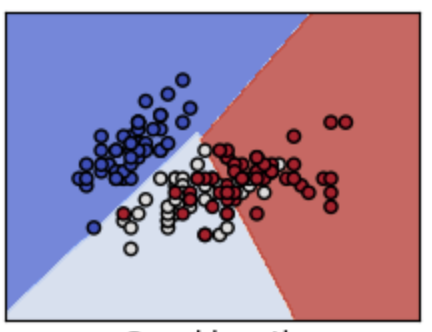
\includegraphics[scale=0.4]{imagenes/Entrenamiento/klineal.png}
        \caption{Kernel lineal}
        \label{fig:cp5:klineal}
        \end{subfigure}%
        \begin{subfigure}{.25\textwidth}
        \centering
        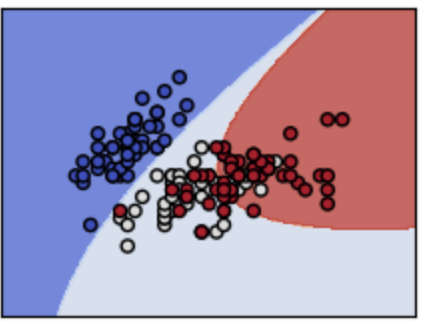
\includegraphics[scale=0.4]{imagenes/Entrenamiento/kpoli.png}
        \caption{Kernel polinomial}
        \label{fig:cp5:kpoli}
        \end{subfigure}%
    
        \begin{subfigure}{.25\textwidth}
        \centering
        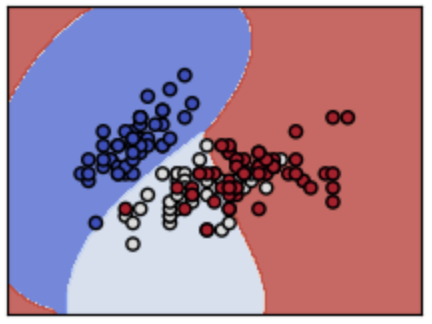
\includegraphics[scale=0.4]{imagenes/Entrenamiento/krbf.png}
        \caption{Kernel radial}
        \label{fig:cp5:krbf}
        \end{subfigure}
      \caption{Kernel de la función [5]}
    \end{figure}


  \end{itemize}


  \item \textbf{Selección}: Los resultados de la sección anterior ha mostrado que no existe una brecha muy grande en el \textbf{exactitud} obtenido de los mejores parámetros, como se muestra en la siguiente Tabla (\ref{tab:cp5:resultados}), como se observa el mejor resultado se ha conseguido con el algoritmo \textbf{Máquina de soporte vectorial} con los parámetros ;$C$=100, $gamma$=0.0001 y $kernel$= $rbf$ (radial) obteniendo 0.8619 de \textbf{exactitud}, por esta razón se ha elegido como el clasificador utilizado en la aplicación.

    \begin{table}[h]
    \centering
      \begin{tabular}{|l|c|c|}
      %-----------------------Ecanbezado-----------------------------------%
        \hline
    \multicolumn{1}{| >{\columncolor{myBlueChapter}}l|}{ \textcolor{myWhite}{\textbf{Algoritmo}} }&
    \multicolumn{1}{| >{\columncolor{myBlueChapter}}l|}{ \textcolor{myWhite}{\textbf{Exactitud}} }&
    \multicolumn{1}{| >{\columncolor{myBlueChapter}}l|}{ \textcolor{myWhite}{\textbf{Ranking}} }
    \\  \cline{1-3}
      %--------------

    MSV&0.8692&1\\
    \hline
    Regresión Logística&0.8682&2\\
    \hline
    Random Forest&0.8619&3\\
    \hline
    Naive Bayes&0.8511&4\\
    \hline
      \end{tabular}
    \caption{Exactitud de los clasificadores}
    \label{tab:cp5:resultados}
    \end{table}

  \item \textbf{Pruebas}: Con base en el algoritmo elegido y los parámetros que han conseguido obtener el mejor resultado, se ha hecho una prueba final, la cual consiste en clasificar el corpus de prueba con 350 noticias, creado al final de la sección de pre-procesamiento, para calcular la matriz de confusión y obtener las métricas de evaluación. La tabla \ref{tab:cp5:numnoticias} muestra el número de noticias por sección contenidas en el corpus.

  \begin{table}[h]
    \centering
      \begin{tabular}{|l|c|}
      %-----------------------Ecanbezado-----------------------------------%
        \hline
    \multicolumn{1}{| >{\columncolor{myBlueChapter}}l|}{ \textcolor{myWhite}{\textbf{Sección}} }&
    \multicolumn{1}{| >{\columncolor{myBlueChapter}}l|}{ \textcolor{myWhite}{\textbf{Número de noticias}} }
    \\  \cline{1-2}
      %--------------

    Deportes& 68\\
    \hline
    Economía& 58\\
    \hline
    Política& 69\\
    \hline
    Cultura& 77\\
    \hline
    Ciencia y Tecnología& 78\\
    \hline
      \end{tabular}
    \caption{Número de noticias}
    \label{tab:cp5:numnoticias}
  \end{table}

  La matriz de confusión obtenida se muestra en la tabla \ref{tab:cp5:matriz}, donde las filas representan la clasificación real de la noticia y las columnas lo predicho por el clasificador. 


  \begin{table}[h]
  \centering
  \resizebox{\columnwidth}{!}{%
    \begin{tabular}{|l|c|c|c|c|c|}
    %-----------------------Ecanbezado-----------------------------------%
      \hline
  \multicolumn{1}{| >{\columncolor{myBlueChapter}}l|}{ \textcolor{myWhite}{\textbf{Sección}} }&
  \multicolumn{1}{| >{\columncolor{myBlueChapter}}l|}{ \textcolor{myWhite}{\textbf{Deportes}} }&
  \multicolumn{1}{| >{\columncolor{myBlueChapter}}l|}{ \textcolor{myWhite}{\textbf{Economía}} }&
  \multicolumn{1}{| >{\columncolor{myBlueChapter}}l|}{ \textcolor{myWhite}{\textbf{Política}} }&
  \multicolumn{1}{| >{\columncolor{myBlueChapter}}l|}{ \textcolor{myWhite}{\textbf{Cultura}} }&
  \multicolumn{1}{| >{\columncolor{myBlueChapter}}l|}{ \textcolor{myWhite}{\textbf{Cienci y T}} }
  \\  \cline{1-6}
    %--------------

  Deportes& 65 & 1 & 1 & 0 & 1\\
  \hline
  Economía& 1 & 51 & 4 & 1 & 1\\
  \hline
  Política& 2 & 5 & 59 & 3 & 0\\
  \hline
  Cultura& 1 & 1 & 1 & 70 & 4\\
  \hline
  Ciencia y T& 1 & 5 & 3 & 2 & 67\\
  \hline
    \end{tabular}
  }
  \caption{Matriz de confusión}
  \label{tab:cp5:matriz}
  \end{table}

  Con base en la matriz de confusión se ha calculado \textbf{Recall}, \textbf{Fmeasure}, \textbf{Precision}. Las métricas son obtenidas por cada sección, como se muestra en la tabla \ref{tab:cp5:metricas}.


  \begin{table}[h]
    \centering
      \begin{tabular}{|l|c|c|c|}
      %-----------------------Ecanbezado-----------------------------------%
        \hline
    \multicolumn{1}{| >{\columncolor{myBlueChapter}}l|}{ \textcolor{myWhite}{\textbf{Sección}} }&
    \multicolumn{1}{| >{\columncolor{myBlueChapter}}l|}{ \textcolor{myWhite}{\textbf{Precision}} }&
    \multicolumn{1}{| >{\columncolor{myBlueChapter}}l|}{ \textcolor{myWhite}{\textbf{Recall}} }&
    \multicolumn{1}{| >{\columncolor{myBlueChapter}}l|}{ \textcolor{myWhite}{\textbf{F-measuere}} }
    \\  \cline{1-4}
      %--------------

    Deportes & 0.93 & 0.96 & 0.94\\
    \hline
    Economía & 0.81 & 0.88 & 0.84\\
    \hline
    Política & 0.87 & 0.86 & 0.86\\
    \hline
    Cultura & 0.92 & 0.91 & 0.92\\
    \hline
    Ciencia y Tecnología & 0.92 & 0.86 & 0.89\\
    \hline
      \end{tabular}
    \caption{Metricas de evaluación}
    \label{tab:cp5:metricas}
  \end{table}


  \item \textbf{Persistencia de modelo}: Como última etapa de la clasificación, el modelo \textbf{Máquina de soporte vectorial} debe ser almacenado así como las características del corpus. Para esta tarea se ha utilizado el corpus completo de 3,500 noticias, del cual se extraen las características, se entrena el modelo y estos conjuntos son almacenados en un archivo ocupando la biblioteca \textbf{pickle}, de esta forma en la siguiente sección el modelo es utilizado como parte de la \textbf{Aplicación web}.

\end{enumerate}
